%%%%%%%%%%%%%%%%%%%%%%%%%%%%%%%%%%%%%%%%%
% Masters/Doctoral Thesis
%
%
% %%%%% IMPORTANT %%%%%
% 1) Edit Front/vars.tex
% 2) Compile Front/main.tex
%
% BEFORE ANYTHING ELSE


%%%%%%%%%%%%%%%%%%%%%%%%%%%%%%%%%%%%%%%%%

%----------------------------------------------------------------------------------------
%	PACKAGES AND OTHER DOCUMENT CONFIGURATIONS
%----------------------------------------------------------------------------------------

\documentclass[11pt, twoside, table,xcdraw]{Thesis} % The default font size and two-sided printing
% For a one-sided printing change the flag "twoside" to "oneside"

\usepackage{pdfpages}
\usepackage[square, numbers, comma, sort&compress]{natbib} % Use the natbib reference package - read up on this to edit the reference style; if you want text (e.g. Smith et al., 2012) for the in-text references (instead of numbers), remove 'numbers'
\usepackage[portuguese,english]{babel}
\usepackage{url} %decent url breaking
\def\UrlBreaks{\do\/\do-}
\usepackage[section]{placeins} %for \FloatBarrier
\usepackage{lipsum} % For dummy text
\usepackage{graphicx}
\usepackage{caption}
\usepackage{subcaption}
\usepackage{fancybox}
\usepackage{ragged2e}
\usepackage{amsmath}
\usepackage{amssymb}
\usepackage{braket}
\usepackage[bottom, perpage, symbol]{footmisc}
\usepackage{csquotes} %added for \begin{displayquote}
\usepackage{verbatim} %added for \begin{comment}
\usepackage{epigraph, varwidth} %added for fancy chapter start quotes
\usepackage{wrapfig} %added for text wrapped around pictures https://pt.sharelatex.com/learn/Wrapping_text_around_figures
\usepackage{listings} %for code listings
\usepackage{color}
\usepackage{multirow}
\usepackage{pdfpages}
\usepackage{algpseudocode}
\usepackage{xargs}    % Use more than one optional parameter in a new commands
\usepackage[colorinlistoftodos,prependcaption,textsize=tiny, textwidth=3cm]{todonotes}
\usepackage{notoccite}
\usepackage{hyperref}
\usepackage{wrapfig}
\usepackage{lipsum}
%\usepackage[hyperpageref]{backref}
%\renewcommand*{\backref}[1]{}
%\renewcommand*{\backrefalt}[4]{
% \ifcase #1
% Not cited.
% \or
% Cited on page~#2.
% \else
% Cited on pages~#2.
% \fi
%}
\hypersetup{colorlinks,citecolor=blue,urlcolor=blue,linkcolor=blue, breaklinks=true}
%%% FONT PACKAGES
% - fourier
% - mathpazo ( palatino for Computer Modern on math )
\usepackage{mathpazo}
\setstretch{1.5}

\graphicspath{{Figures/}} % Specifies the directory where pictures are stored

%%% BIB STYLE
%\bibliographystyle{apsrev4-1-etal} % With emphasized titles. ORIGINAL
%\bibliographystyle{apsrev4-1} %this one isn't available, for some reason
\bibliographystyle{IEEEtranN}


\definecolor{dkgreen}{rgb}{0,0.6,0}
\definecolor{gray}{rgb}{0.5,0.5,0.5}
\definecolor{mauve}{rgb}{0.58,0,0.82}
\definecolor{codegreen}{rgb}{0,0.6,0}
\definecolor{codegray}{rgb}{0.5,0.5,0.5}
\definecolor{codepurple}{rgb}{0.58,0,0.82}
\definecolor{backcolour}{rgb}{0.95,0.95,0.92}
\definecolor{orange}{RGB}{255,127,0}

\lstdefinestyle{Python}{
        language=Python,
         numberstyle=\small,
         stepnumber=2,
         numbersep=10pt,
         basicstyle={\small\ttfamily},
         keywordstyle    = \color{blue},
         commentstyle    = \color{red}\ttfamily,
         stringstyle=\color{orange},
         tabsize=2,
         columns=fullflexible,
         backgroundcolor=\color{backcolour},
         frame=none,
         numbers=left,
         aboveskip=5mm,
         belowskip=5mm,
         breaklines=true
}

%Overload epigraph command
\renewcommand{\epigraphsize}{\small}
\setlength{\epigraphwidth}{0.90\textwidth}
\renewcommand{\textflush}{flushright}
\renewcommand{\sourceflush}{flushright}
% A useful addition
\newcommand{\epitextfont}{\itshape}
\newcommand{\episourcefont}{\scshape}

\makeatletter
\newsavebox{\epi@textbox}
\newsavebox{\epi@sourcebox}
\newlength\epi@finalwidth
\renewcommand{\epigraph}[2]{%
  \vspace{\beforeepigraphskip}
  {\epigraphsize\begin{\epigraphflush}
   \epi@finalwidth=\z@
   \sbox\epi@textbox{%
     \varwidth{\epigraphwidth}
     \begin{\textflush}\epitextfont#1\end{\textflush}
     \endvarwidth
   }%
   \epi@finalwidth=\wd\epi@textbox
   \sbox\epi@sourcebox{%
     \varwidth{\epigraphwidth}
     \begin{\sourceflush}\episourcefont#2\end{\sourceflush}%
     \endvarwidth
   }%
   \ifdim\wd\epi@sourcebox>\epi@finalwidth
     \epi@finalwidth=\wd\epi@sourcebox
   \fi
   \leavevmode\vbox{
     \hb@xt@\epi@finalwidth{\hfil\box\epi@textbox}
     \vskip1.75ex
     \hrule height \epigraphrule
     \vskip.75ex
     \hb@xt@\epi@finalwidth{\hfil\box\epi@sourcebox}
   }%
   \end{\epigraphflush}
   \vspace{\afterepigraphskip}}}
\makeatother
%End of overload command


\DeclareMathAlphabet{\pazocal}{OMS}{zplm}{m}{n}
\newcommand{\Sa}{\pazocal{S}}
\newcommand{\Ua}{\pazocal{U}}
\newcommand{\Ha}{\pazocal{H}}
\newcommand{\Fa}{\pazocal{F}}
\newcommand{\Ia}{\pazocal{I}}
\newcommand{\Ea}{\pazocal{E}}
\newcommand{\ja}{\pazocal{J}}


\renewcommand{\labelitemi}{$\bullet$}


\setlength{\headheight}{14pt}  %Try fix error

%Custom hyphenization
\hyphenation{Py-thon}
\hyphenation{Ju-py-ter}
\hyphenation{Ma-the-ma-ti-ca}

%Custom math operators
\DeclareMathOperator*{\meshgrid}{meshgrid}

% floor and ceiling of numbers
\usepackage{mathtools}
\DeclarePairedDelimiter\ceil{\lceil}{\rceil}
\DeclarePairedDelimiter\floor{\lfloor}{\rfloor}

% ---------------------------------------------------------------------------------
%   Notes on the documents!!!
% https://tex.stackexchange.com/questions/9796/how-to-add-todo-notes
% https://tex.stackexchange.com/questions/316220/todo-commentsnot-include-and-left-align
% EXAMPLES:
%\unsure{Is this correct?}\unsure{I'm unsure about also!}
%\change{Change this!}
%\info{This can help me in chapter seven!}
%\improvement{This really needs to be improved!\newline\newline What was I thinking?!}
% \thiswillnotshow{This is hidden since option `disable' is chosen!}
% WARNING: It eliminates whitespaces in front of it. You can add trailing {} to avoid
%\usepackage{xargs}    % Use more than one optional parameter in a new commands
%\usepackage[colorinlistoftodos,prependcaption,textsize=tiny, textwidth=3cm]{todonotes}

\newcommandx{\unsure}[2][1=]{\setlength{\marginparwidth}{3cm}\reversemarginpar\todo[linecolor=red,backgroundcolor=red!25,bordercolor=red,#1]{#2}}

\newcommandx{\change}[2][1=]{\setlength{\marginparwidth}{3cm}\reversemarginpar\todo[linecolor=blue,backgroundcolor=blue!25,bordercolor=blue,#1]{#2}}

\newcommandx{\info}[2][1=]{\setlength{\marginparwidth}{3cm}\reversemarginpar\todo[linecolor=green,backgroundcolor=green!25,bordercolor=green,#1]{#2}}

\newcommandx{\improvement}[2][1=]{\setlength{\marginparwidth}{3cm}\reversemarginpar\todo[linecolor=yellow,backgroundcolor=yellow!25,bordercolor=yellow,#1]{#2}}

\newcommandx{\thiswillnotshow}[2][1=]{\setlength{\marginparwidth}{3cm}\reversemarginpar\todo[disable,#1]{#2}}
%


%----------------------------------------------------------------------------------------
%	DOCUMENT VARIABLES
%----------------------------------------------------------------------------------------

\thesistitle{MyThesis Title} % Your thesis title \ttitle
\thesistype{Masters Thesis} % Your thesis type Doctoral Thesis or Masters Thesis \ttype
\supervisor[mailto:example@fc.up.pt]{FirstName \textsc{LastName}} % Your s.upervisor's name \supname \supnamenolink
%\cosupervisor[mailto:name@host.com]{John \textsc{Doe}} % Your supervisor's name \cosupname \cosupnamenolinkTo
% To hide the Co-Supervisor field, just comment out \cosupervisor
\degree{MSc. Engineering Physics} % Your degree name \degreename
\authors[mailto:example@fc.up.pt]{MyName \textsc{MyLastName}} % Your name \authornames \authornamesnolink
\addresses{} % Your address \addressname
\subject{Physics} % Your subject area \subjectname
\keywords{physics} % Keywords for your thesis \keywordnames
\university{Universidade do Porto} % Your university's name \univname \univnamenolink
\UNIVERSITY{UNIVERSIDADE DO PORTO} % Your university's name in capitals \UNIVNAME \UNIVNAMEnolink
\department{Departamento de Física e Astronomia} % Your department's name \deptname \deptnamenolink
\DEPARTMENT{DEPARTAMENTO DE FÍSICA E ASTRONOMIA} % Your department's name in capitals \DEPTNAME \DEPTNAMEnolink
% To hide the Department field, just comment out \DEPARTMENT and \department
%\group[http://www.groupurl.com]{Research Group} % Your research group's name \groupname \groupnamenolink
%GROUP[http://www.groupurl.com]{RESEARCH GROUP} % Your research group's name in capitals \GROUPNAME \GROUPNAMEnolink
% To hide the Group field, just comment out \GROUP and \group
\faculty{Faculdade de Ciências da Universidade do Porto} % Your faculty's name \facname \facnamenolink
\FACULTY{FACULDADE DE CIÊNCIAS DA UNIVERSIDADE DO PORTO} % Your faculty's name in capitals \FACNAME \FACNAMEnolink
% To hide the Faculty field, just comment out \FACULTY and \Faculty
% NOTE: To remove links write \cmd{name} instead of \cmd[link]{name}
% NOTE: For aesthetics, at least one of these fields must be set: faculty, group or department


%----------------------------------------------------------------------------------------
%	NOTATION VARIABLES
%----------------------------------------------------------------------------------------

\newcommand{\dd}{\mathrm{d}}


%----------------------------------------------------------------------------------------
%	DOCUMENT
%----------------------------------------------------------------------------------------

\begin{document}

\pagestyle{empty}
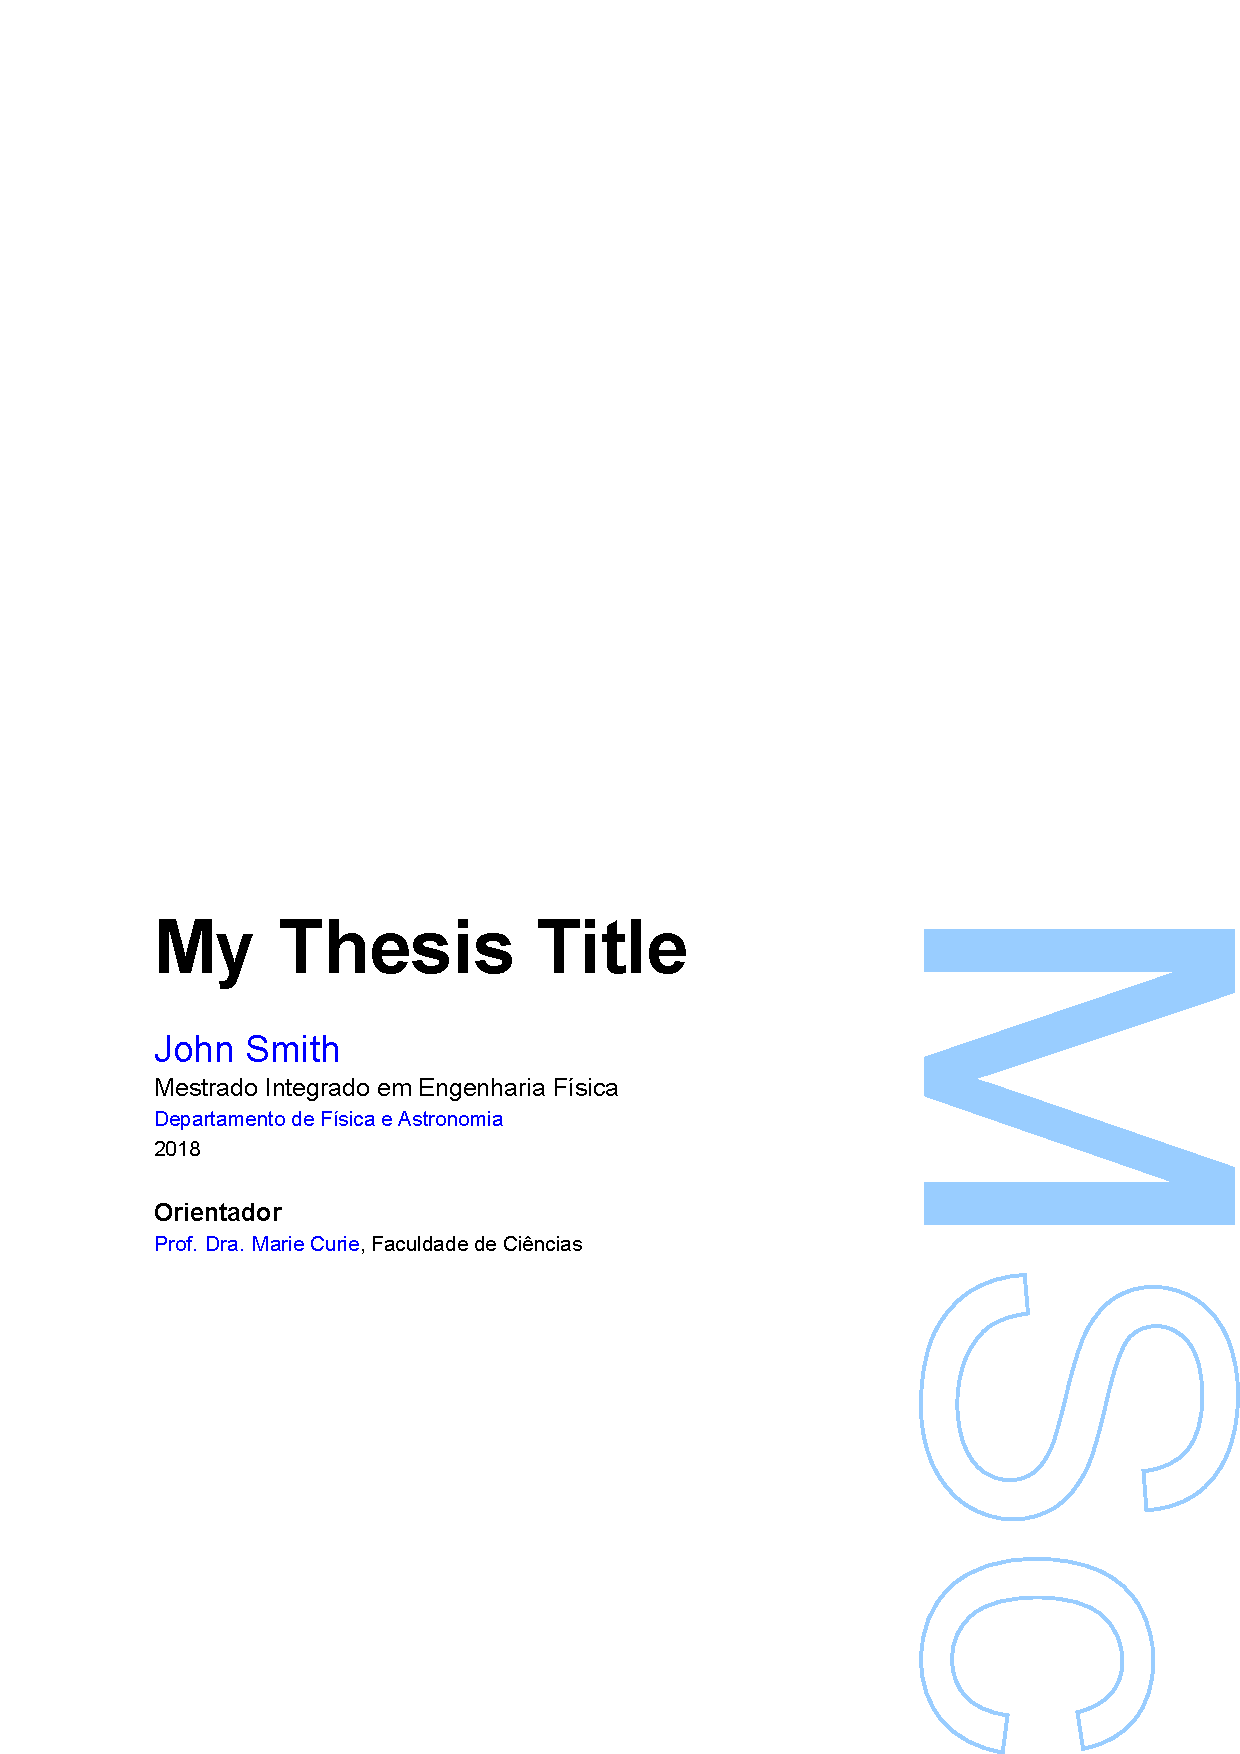
\includepdf[pages={1},pagecommand={},scale=1]{Front/main}
\cleardoublepage
\includepdf[pages={2},pagecommand={},scale=1]{Front/main}
\cleardoublepage
\pagestyle{fancy}


\frontmatter % Use roman page numbering style (i, ii, iii, iv...) for the pre-content pages


%----------------------------------------------------------------------------------------
%	TITLE PAGE
%----------------------------------------------------------------------------------------

\maketitle

%----------------------------------------------------------------------------------------
%	QUOTATION PAGE
%----------------------------------------------------------------------------------------

\quotepage{Matt Smith as \emph{The Doctor}, written by Matthew Graham}
{
	I am and always will be the optimist, the hoper of far-flung hopes and the dreamer of \newline improbable dreams
}


%----------------------------------------------------------------------------------------
%	ACKNOWLEDGEMENTS
%----------------------------------------------------------------------------------------
\begin{acknowledgements}

Acknowledge ALL the people!

\end{acknowledgements}

\addvspacetoc{0.3cm} % Add a gap in the Contents, for aesthetics


%----------------------------------------------------------------------------------------
%	ABSTRACT PAGE
%----------------------------------------------------------------------------------------
\begin{abstract}

This thesis is about something, I guess....

\end{abstract}

%----------------------------------------------------------------------------------------
%	ABSTRACT PAGE (PORTUGUESE)
%----------------------------------------------------------------------------------------
\begin{abstract}[
	thesistitle={Titulo da Tese em Portugês},
	title={Resumo},
	degree={Mestrado Integrado em Engenharia Física},
	nameconnector={por}]
\begin{otherlanguage}{portuguese}

Este tese é sobre alguma coisa

\end{otherlanguage}
\end{abstract}

%----------------------------------------------------------------------------------------
%	LIST OF CONTENTS/FIGURES/TABLES
%----------------------------------------------------------------------------------------

\addvspacetoc{0.3cm}

\tableofcontents % Write out the Table of Contents

\listoffigures % Write out the List of Figures

%\listoftables % Write out the List of Tables

%\addvspacetoc{0.3cm}

%----------------------------------------------------------------------------------------
%	PHYSICAL CONSTANTS/OTHER DEFINITIONS
%----------------------------------------------------------------------------------------

%\begin{listofcontants}
%	\const{My little ponny test of magical rainbow}{$mn/mp$}{$2.997\ 924\ 58\times10^{8}\ \mbox{ms}^{-\mbox{s}}$}
%	\const{Vaccuum permeability test of magical rainbow for a specific case of condensed matter physics}{$\epsilon_0$}{$2.997\ 924\ 58\times10^{8}\ \mbox{ms}^{-\mbox{s}}$}
%	\const{Speed of Light test of magical rainbow}{$c$}{$2.997\ 924\ 58\times10^{8}\ \mbox{ms}^{-\mbox{s}}$}
%\end{listofcontants}


%----------------------------------------------------------------------------------------
%	SYMBOLS
%----------------------------------------------------------------------------------------

%\begin{listofsymbols}
%	\symb{$F_{\mu\nu}$}{Maxwell tensor}{F}
%	\symb{$a$}{distance}{m}
%	\\
%	\symb{$\omega$}{angular frequency}{rads$^{-1}$}
%\end{listofsymbols}


%----------------------------------------------------------------------------------------
%	NOTATION
%----------------------------------------------------------------------------------------

% \newcommand\notationname{Notation and Conventions}
% \addtotoc{\notationname}
% \fancyhead[LO]{\textsc{\notationname}}

% \input{Notation}



%----------------------------------------------------------------------------------------
%	ABBREVIATIONS
%----------------------------------------------------------------------------------------

%\begin{glossary}
%	\abbrev{QM}{Quantum Mechanics}
%\end{glossary}


%----------------------------------------------------------------------------------------
%	DEDICATORY
%----------------------------------------------------------------------------------------

%\begin{dedicatory}
%	This thesis is dedicated to my family, for their love and support.
%\end{dedicatory}


%----------------------------------------------------------------------------------------
%	THESIS CONTENT - CHAPTERS
%----------------------------------------------------------------------------------------

\addvspacetoc{0.3cm}

\mainmatter % Begin numeric (1,2,3...) page numbering

\pagestyle{fancy}
\renewcommand{\chaptermark}[1]{\markboth{\thechapter. \textsc{#1}}{}}
\fancyhead[LO]{\leftmark}

%%% -----------  ADD CHAPTERS HERE ------------------ %%%

% Chapter Template


\chapter{Chapter Title Here} % Main chapter title
%\chapter[toc version]{doc version}
%\chaptermark{version for header} %Short version of the title for the headeer
\label{ChapterX} % Change X to a consecutive number; for referencing this chapter elsewhere, use \ref{ChapterX}

% Write text in here
% Use \subsection and \subsubsection to organize text
Chapter contets here.

Lorem ipsum dolor sit amet, pri ut diam esse, iudico fierent pertinacia vim ad, cu affert deleniti invenire sed. Elitr luptatum repudiandae ut eos. An pri eros mucius legimus, eu wisi noster his. No omnes voluptatibus per, sea at paulo sonet quaerendum, id sea nibh albucius salutatus. Eam ne suas agam voluptatibus, vix at semper intellegat, ut movet verear habemus has \cite{Nobody06}.

Nec ea veri aperiri atomorum, duo probo audire aperiri ne. Utamur percipit id pro, in tota inani pro. Has iuvaret nominati id. Patrioque assueverit pro cu, natum affert exerci qui no. Ne hinc homero mediocrem eum, oblique meliore sea an.

Ex ius illud nihil, no singulis constituto incorrupte mea, nulla insolens ea has. Mea ex nonumy luptatum. Melius volumus no per, at tantas corpora pro. Vis mollis meliore ad, graeci atomorum his id. His ludus atomorum deseruisse ex. Ut mei graece saperet democritum \ref{fig:FCUPfatCat}. 

Nam essent minimum ne, ad nam facilis forensibus. Te scripta omnesque ius. Sale perfecto mediocritatem an vis, ne his unum placerat, cu mei doming cetero delectus. Duo falli iudico concludaturque id, et vim suscipit senserit, qui noster indoctum democritum te. Ut quo paulo legendos expetendis, ut illum harum voluptatibus ius, prima dolores oporteat cu usu.

\begin{figure}
	\centering
	\begin{subfigure}{.49\textwidth}
  		\centering
  		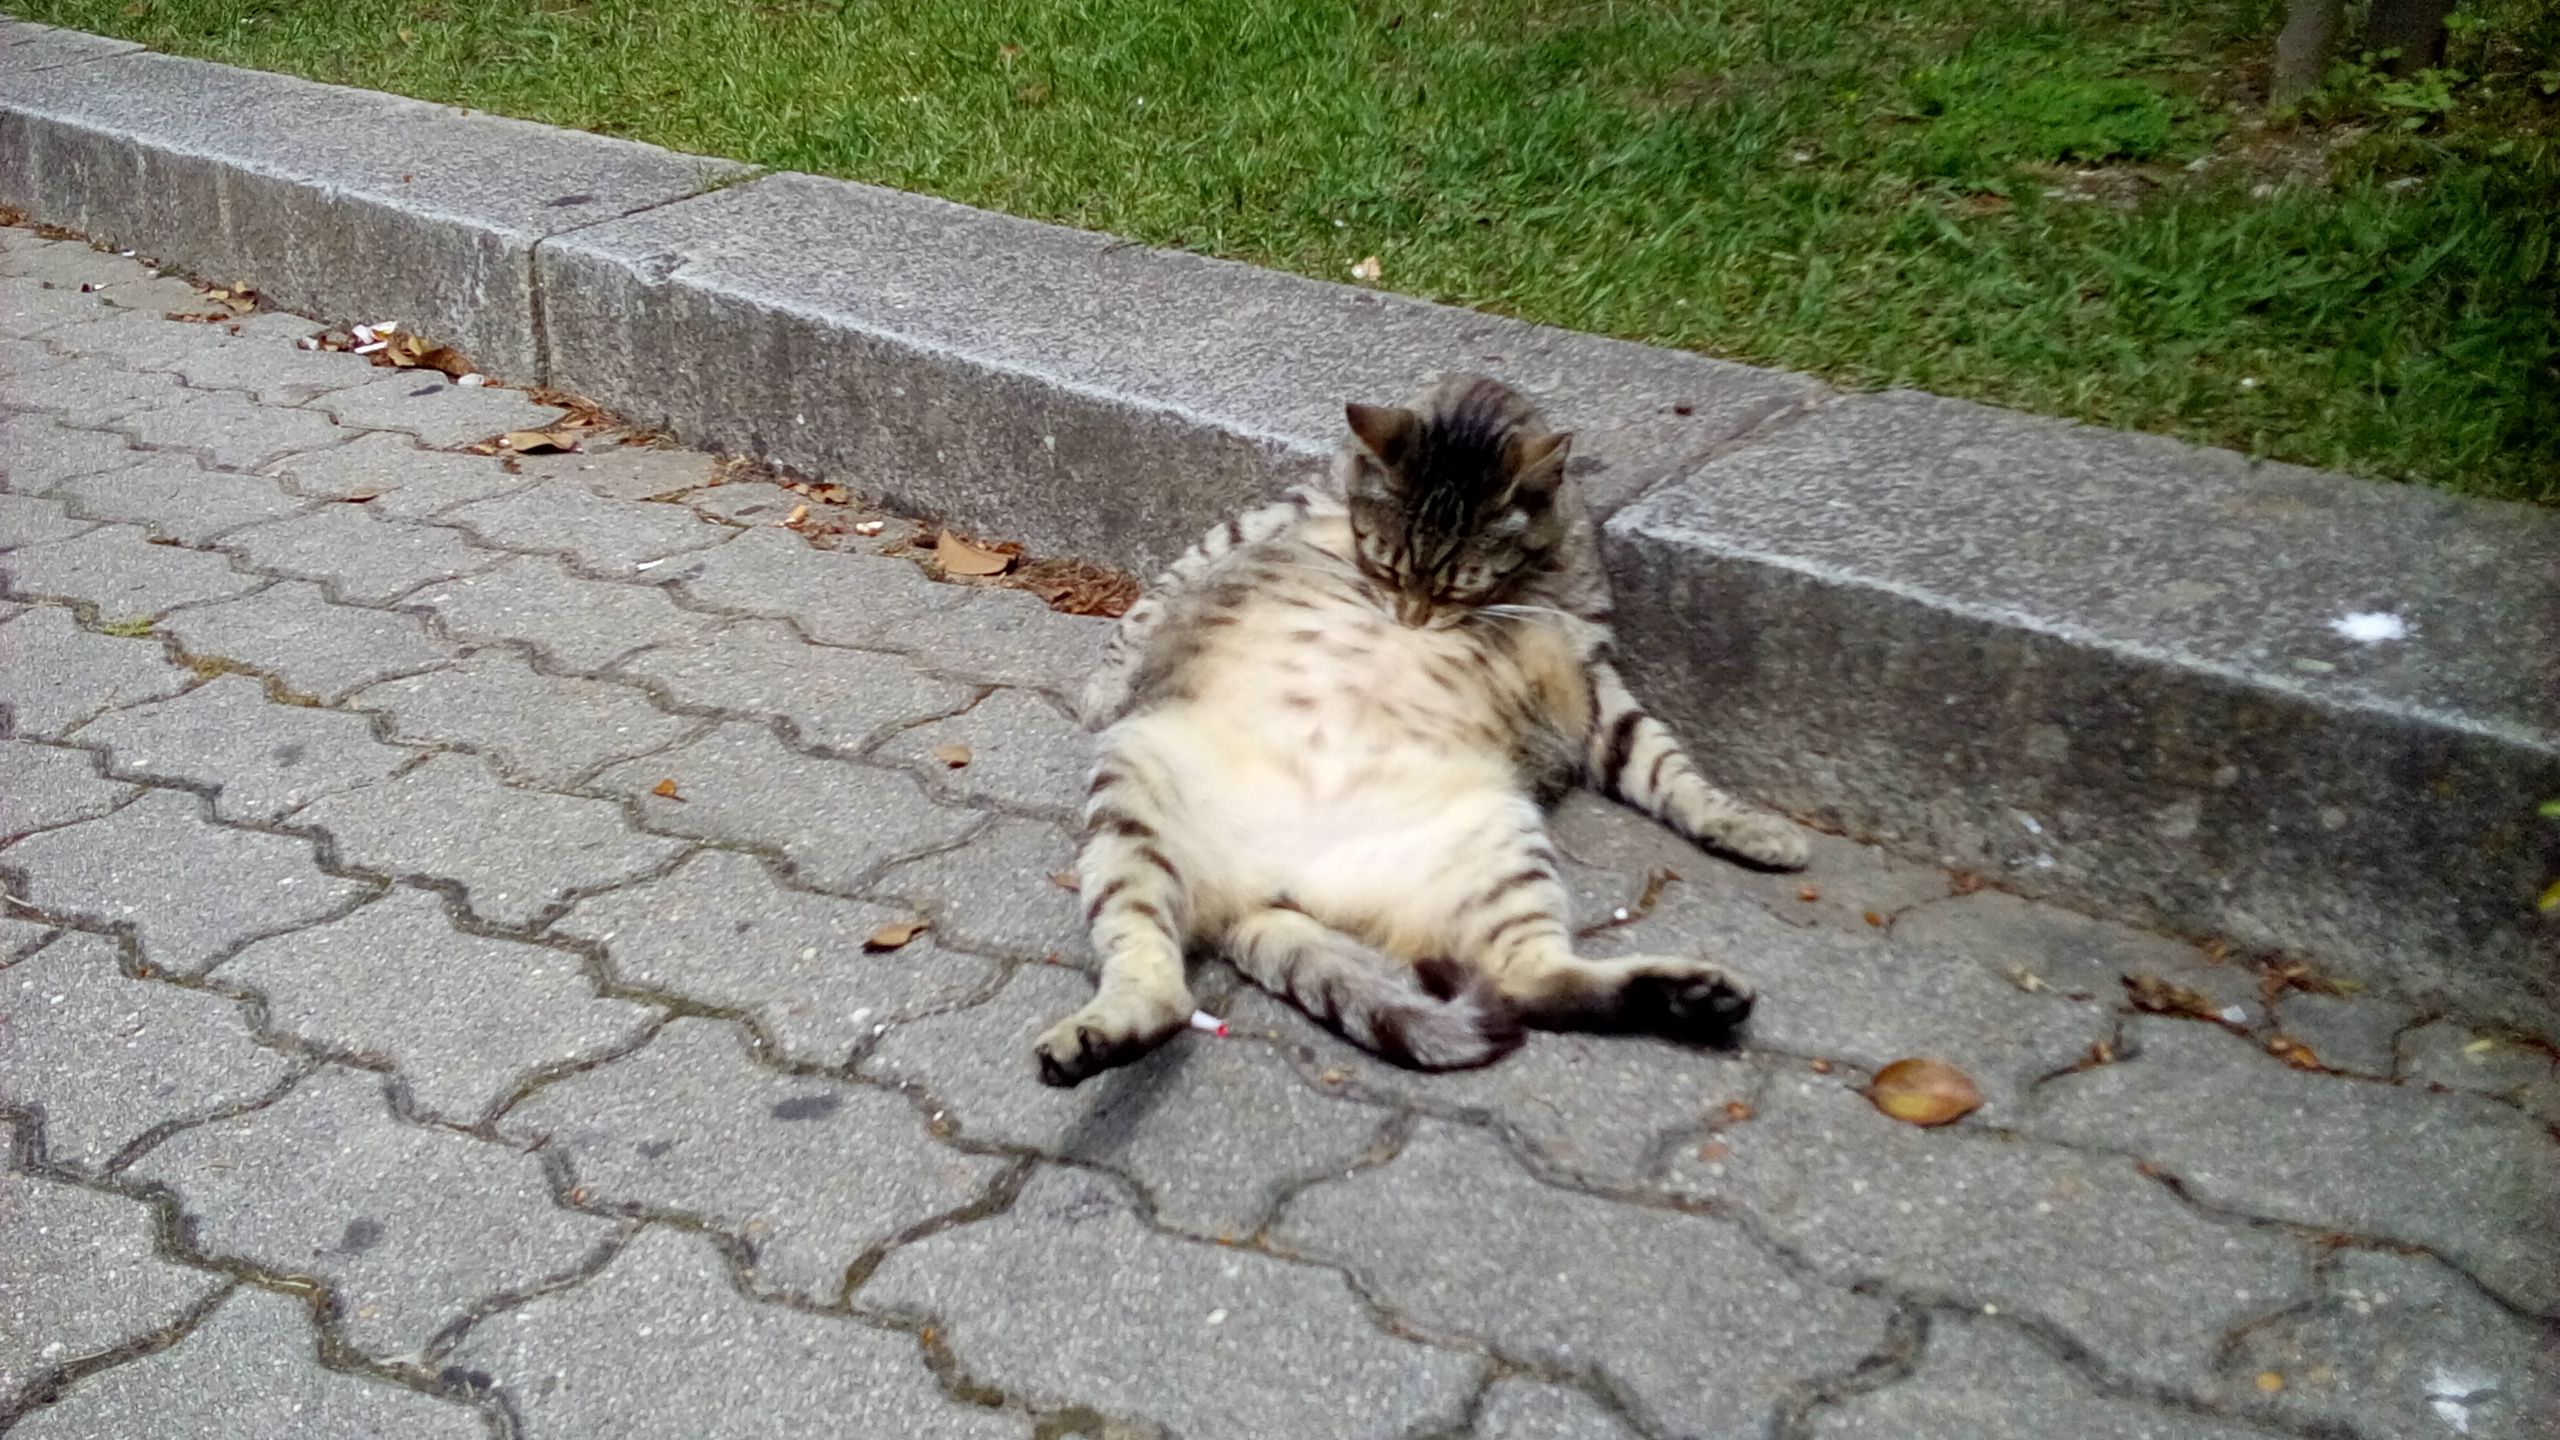
\includegraphics[width=.95\linewidth]{Figures/ChapterTemplate/20160517_123603.jpg}
  		\caption{FCUP's fat cat doing what cats do.}
	\end{subfigure}%
	\hfill
	\begin{subfigure}{.49\textwidth}
  		\centering
 		 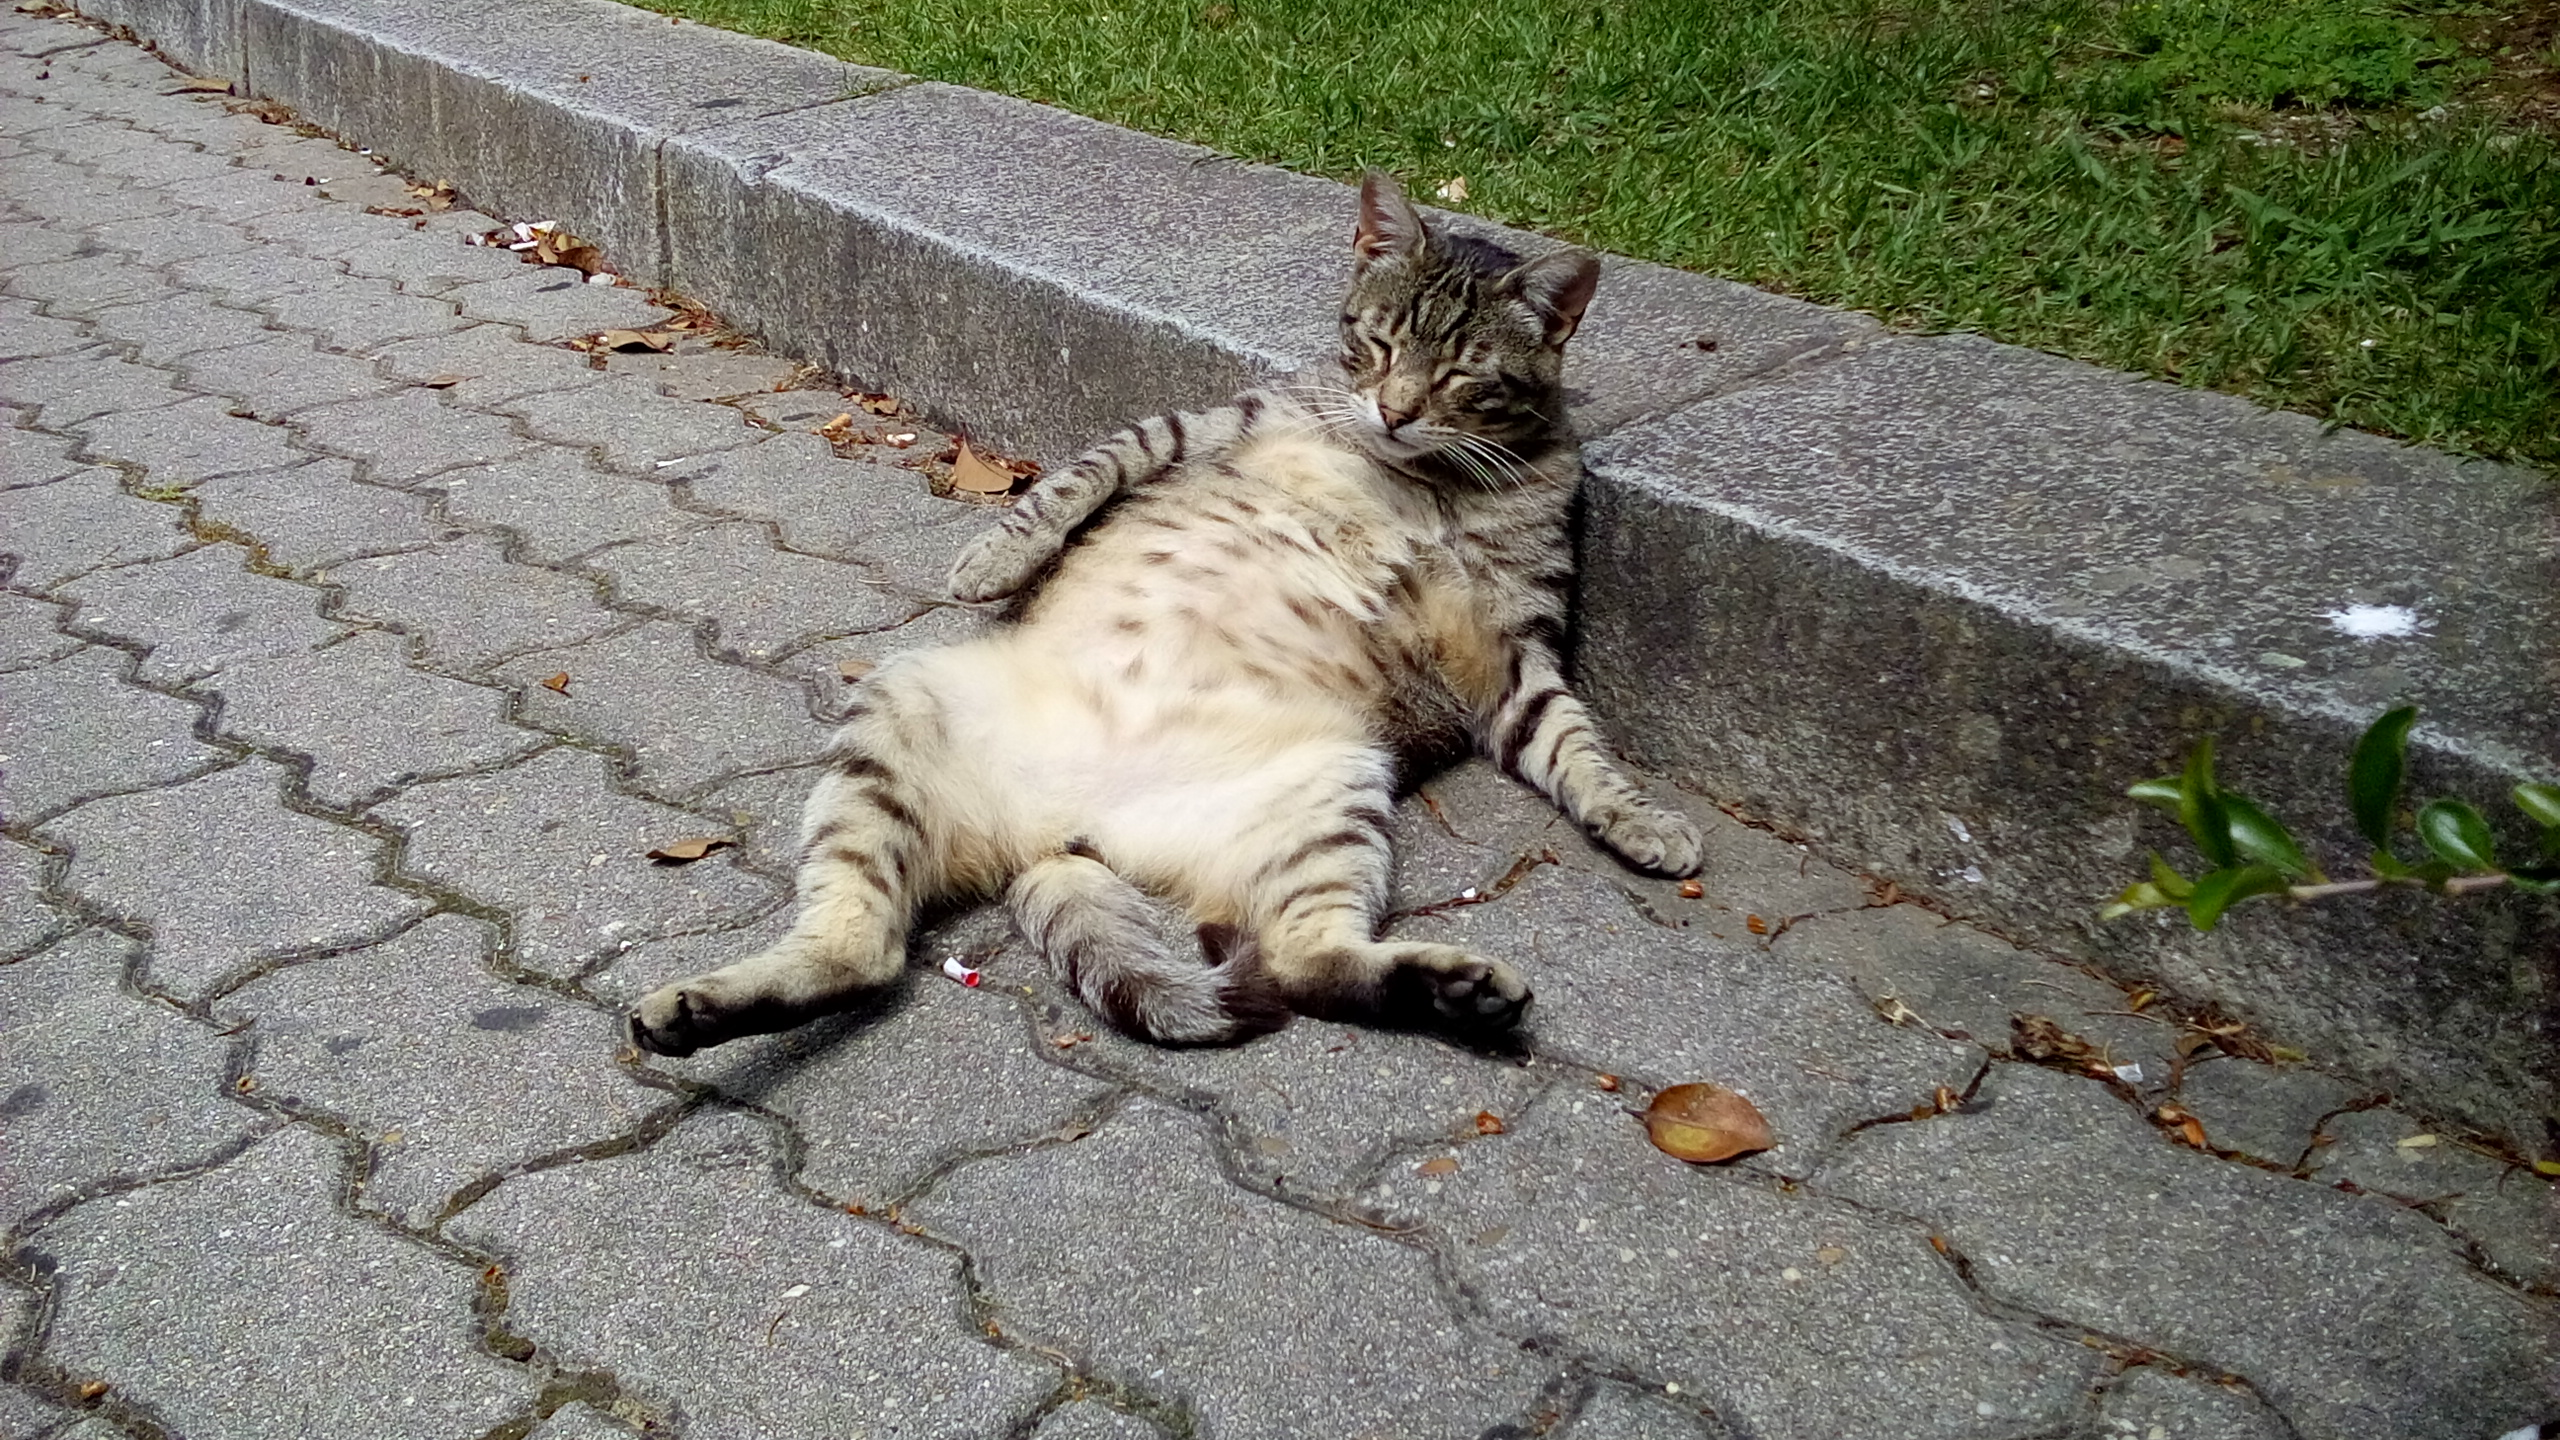
\includegraphics[width=.95\linewidth]{Figures/ChapterTemplate/20160517_123609.jpg}
 		 \caption{FCUP's fat cat resting.}
	\end{subfigure}
	\caption{\label{fig:FCUPfatCat}FCUP's fat cat.} 
\end{figure}

Vix ex alii ponderum percipitur, laudem audiam his at, at dicit delectus sed. No vel affert docendi offendit. Ea quod tincidunt pro. Id clita veniam nam, an his diceret prodesset. Eligendi neglegentur vel et. Ne nobis appareat his, has ei alienum epicurei omittantur, tempor prompta feugait vim at.

Libris comprehensam est ad, eos cu diam atqui. Eos at vide iusto posidonium, omnes tacimates ad mei. Te alii propriae laboramus eos, mea prima timeam fierent ad, nam et nostro efficiantur accommodare. Ad sea probatus phaedrum, case corrumpit sit id, vix ex alterum repudiandae. Duo dolorum euripidis at, cu eos dolores hendrerit temporibus, vel oratio alterum sadipscing ex. Nulla molestie accusata per te, pri percipit rationibus at, vis modo commune te.

Te tantas persecuti mea. Mel et nostrum voluptua, ut duo nisl ludus volumus. Pri agam labitur te. An quis veritus appetere duo, mei laoreet praesent no. Cu quem postea vocent mel, essent eruditi scaevola quo ea.

Ne pri maiestatis quaerendum, ei nec hinc veniam dicunt. Electram concludaturque eos ut. Eam nisl semper ad, ut vix bonorum imperdiet voluptatibus, nam veri fabulas convenire ex. Ad vix dicat noster, agam utamur erroribus ea est, mucius ancillae scriptorem sea eu. Eos ea nominati conclusionemque, usu esse nonumy facilisis cu.

Atqui tamquam eloquentiam ut qui. Pro te offendit honestatis, forensibus vituperatoribus pri ea. Et mea alii eligendi referrentur, primis urbanitas per et. Nec te graeci doctus. Utinam maiorum est at. An iracundia ullamcorper definitionem mea.

Nec alia dicunt te, in malis appareat his. Cu sumo adhuc scripserit nec, usu te mundi decore tamquam. Sea te atomorum laboramus expetendis, virtute gloriatur signiferumque pri et. Nostro eirmod perpetua an mea, id cum graecis persecuti consequuntur, eam volumus singulis scriptorem ut. Has tritani inimicus in, ea zril munere repudiandae pro.

Nam at homero aliquid, has sale etiam dicit ad. Electram argumentum eu eum, usu ne quis aliquando. Ex mei brute vocibus. Et vim dictas iriure oporteat, sea appetere ullamcorper te, ea pro altera tibique. Eam expetendis suscipiantur ea. Velit deserunt volutpat sea cu, tollit facilisi ei vis.

Sed id ignota placerat mediocrem, mel ut semper efficiendi instructior. Ne veri melius volumus vel. Sit elit aliquam cu. Dico tritani disputando id his, natum fugit impedit has no. Nam ex fugit regione. Nam honestatis theophrastus in, ut mei quas graecis blandit. At veniam tempor imperdiet eam, ad ius facer interpretaris.

Eos autem omittantur at. Eum dolorem facilis no, sonet omnium has id. Ea est option fastidii recteque, ne reque malis reformidans mel. Mei commodo civibus persecuti at, ea augue ceteros elaboraret mea, pertinacia omittantur ad sea.

Ne magna debet philosophia qui, fabellas sensibus ex vel, mei ut dicant vidisse molestie. Aliquam denique id usu, vis paulo ubique senserit et, mandamus definiebas scriptorem est no. Ex utinam essent deserunt cum, solum reque torquatos sit ut. Omnis verear imperdiet eum et. Sea hinc ferri libris in. Te error quaestio accommodare cum.

Quem honestatis repudiandae per in, no has eros iracundia. Eum te velit saperet accommodare. Nam in melius integre, solet possim vocibus ad usu. Timeam verterem vulputate ad eam, viris legere aliquid ea vis. Usu ut tation eirmod periculis, ludus deleniti deterruisset eam at. Ea exerci consequuntur nec, facete civibus splendide ex sea.

Sumo vituperata an mea, ut cibo delicata mel. Has audire qualisque et, vero consul fuisset ne his, quo et tollit doctus mnesarchum. Putent maluisset at eos, mel ad everti aliquam, et sit clita electram molestiae. Ius in adhuc animal. Quo id eros mazim iriure, ea per audire minimum omittantur. Id has alii choro incorrupte, solum nonumes ex vel, cu atomorum similique mei.

Viris partiendo instructior pri cu, te cum vitae saperet phaedrum. Mei dolor aperiam accommodare te. Summo pericula mediocrem an cum, debitis hendrerit signiferumque cu vis. Qui ne regione alterum mandamus, autem augue mediocrem eum at. Eum ex discere noluisse postulant, mea ad persecuti reformidans instructior. In his dicam delenit epicurei, porro omittantur vel ad, et mucius sensibus nec.

An mea modus adversarium. Odio facer cum ea. Oblique platonem evertitur ut pro, no assum patrioque similique cum. Nullam viderer mea at, no sale augue sit, aeque decore aliquip mel cu. Vero voluptaria no est, est in sint eius antiopam.

Eam affert exerci omnium et, vis admodum contentiones interpretaris ut. Idque laboramus duo eu. Vide docendi atomorum cu eos. Mea quidam abhorreant at, tale zril disputationi vix ne. Eu adhuc sonet pri, vix nulla dolor at. Ei qui solum molestiae, mea cu vivendo constituam.

Id laboramus definitionem duo. Et elit vocent antiopam eos. Brute facilisi complectitur mel no, timeam habemus omnesque id nam, ius mutat consectetuer ut. Te mel habemus delicata scripserit. Ei fuisset intellegat per. Mei ex duis augue voluptatum.
% Add others as needed



%----------------------------------------------------------------------------------------
%	THESIS CONTENT - APPENDICES
%----------------------------------------------------------------------------------------

\appendix % Cue to tell LaTeX that the following 'chapters' are Appendices

%%% -----------  ADD APPENDIX HERE ------------------ %%%

% Appendix Template

\chapter{Appendix Title Here} % Main appendix title

\label{AppendixX} % Change X to a consecutive letter; for referencing this appendix elsewhere, use \ref{AppendixX}

Write your Appendix content here.
%\input{Appendices/AppendixB}
%\input{Appendices/AppendixC}

\backmatter

%----------------------------------------------------------------------------------------
%	BIBLIOGRAPHY
%----------------------------------------------------------------------------------------

\addvspacetoc{0.5cm}
\addtotoc{Bibliography}

\fancyhead[LO]{\textsc{Bibliography}}

\bibliography{Bibliography} % The references are stored in the file "Bibliography.bib"


\end{document}
